\section{Unrequited Love}\label{chapter:UL1}

\textit{\textbf{Note}: for this section only, we shall use the convention $W = W_{ij} = W_{i \leftarrow j}$ for the transition matrices, such that the stationary probability vector $P_{\infty}$ is now a right eigenvector of $e^{tW}$. In this convention we have $\bra{j}M\ket{i} = M_{ij}$.}

\textit{In this section we derive an expression for the path probabilities of the elusive unrequited love system. We then anticipate an extension of the generating function approach to evaluating these probabilities in closed form.}
\subsection{System Description}

We couple a second Poisson process to a symmetric telegraph process described in Section \ref{chapter:telegraph}. A first particle, call it the leader, jumps independently between states $\ket{1}$ and $\ket{2}$. A second particle, call it the follower, shares this phase space, but it is coupled to the first particle. That is, the probability of a transition $\ket{i} \rightarrow \ket{j}$ for the follower depends on the state of the leader. The phase space of the two particle system is $\mathcal{X} = \{ \ket{11}, \ket{12}, \ket{22}, \ket{21}\}$ where $\ket{x_Ax_B} = \ket{11}$ is the state where both particles are in state $\ket{1}$ of their marginal system and so on. $\ket{x_A}, \ket{x_B}$ denotes the state of the leader and the follower, respectively. The two particle ensemble we shall call the granular Unrequited Love (UL) system. The time evolution of the granular UL system is governed by the master equation

\begin{align}
\dot{P}(t) = e^{tW}P(t), \; \; \;  W = \begin{pmatrix} -\alpha - \beta & \alpha & \beta + \gamma & 0 \\
  \alpha & -\alpha -\beta -\gamma & 0 & \beta \\
  \beta & 0 & -\alpha-\beta-\gamma & \alpha \\
  0 & \beta+\gamma & \alpha & -\alpha-\beta\end{pmatrix}.
\end{align}

\begin{wrapfigure}{R}{0.45\textwidth}
\centering
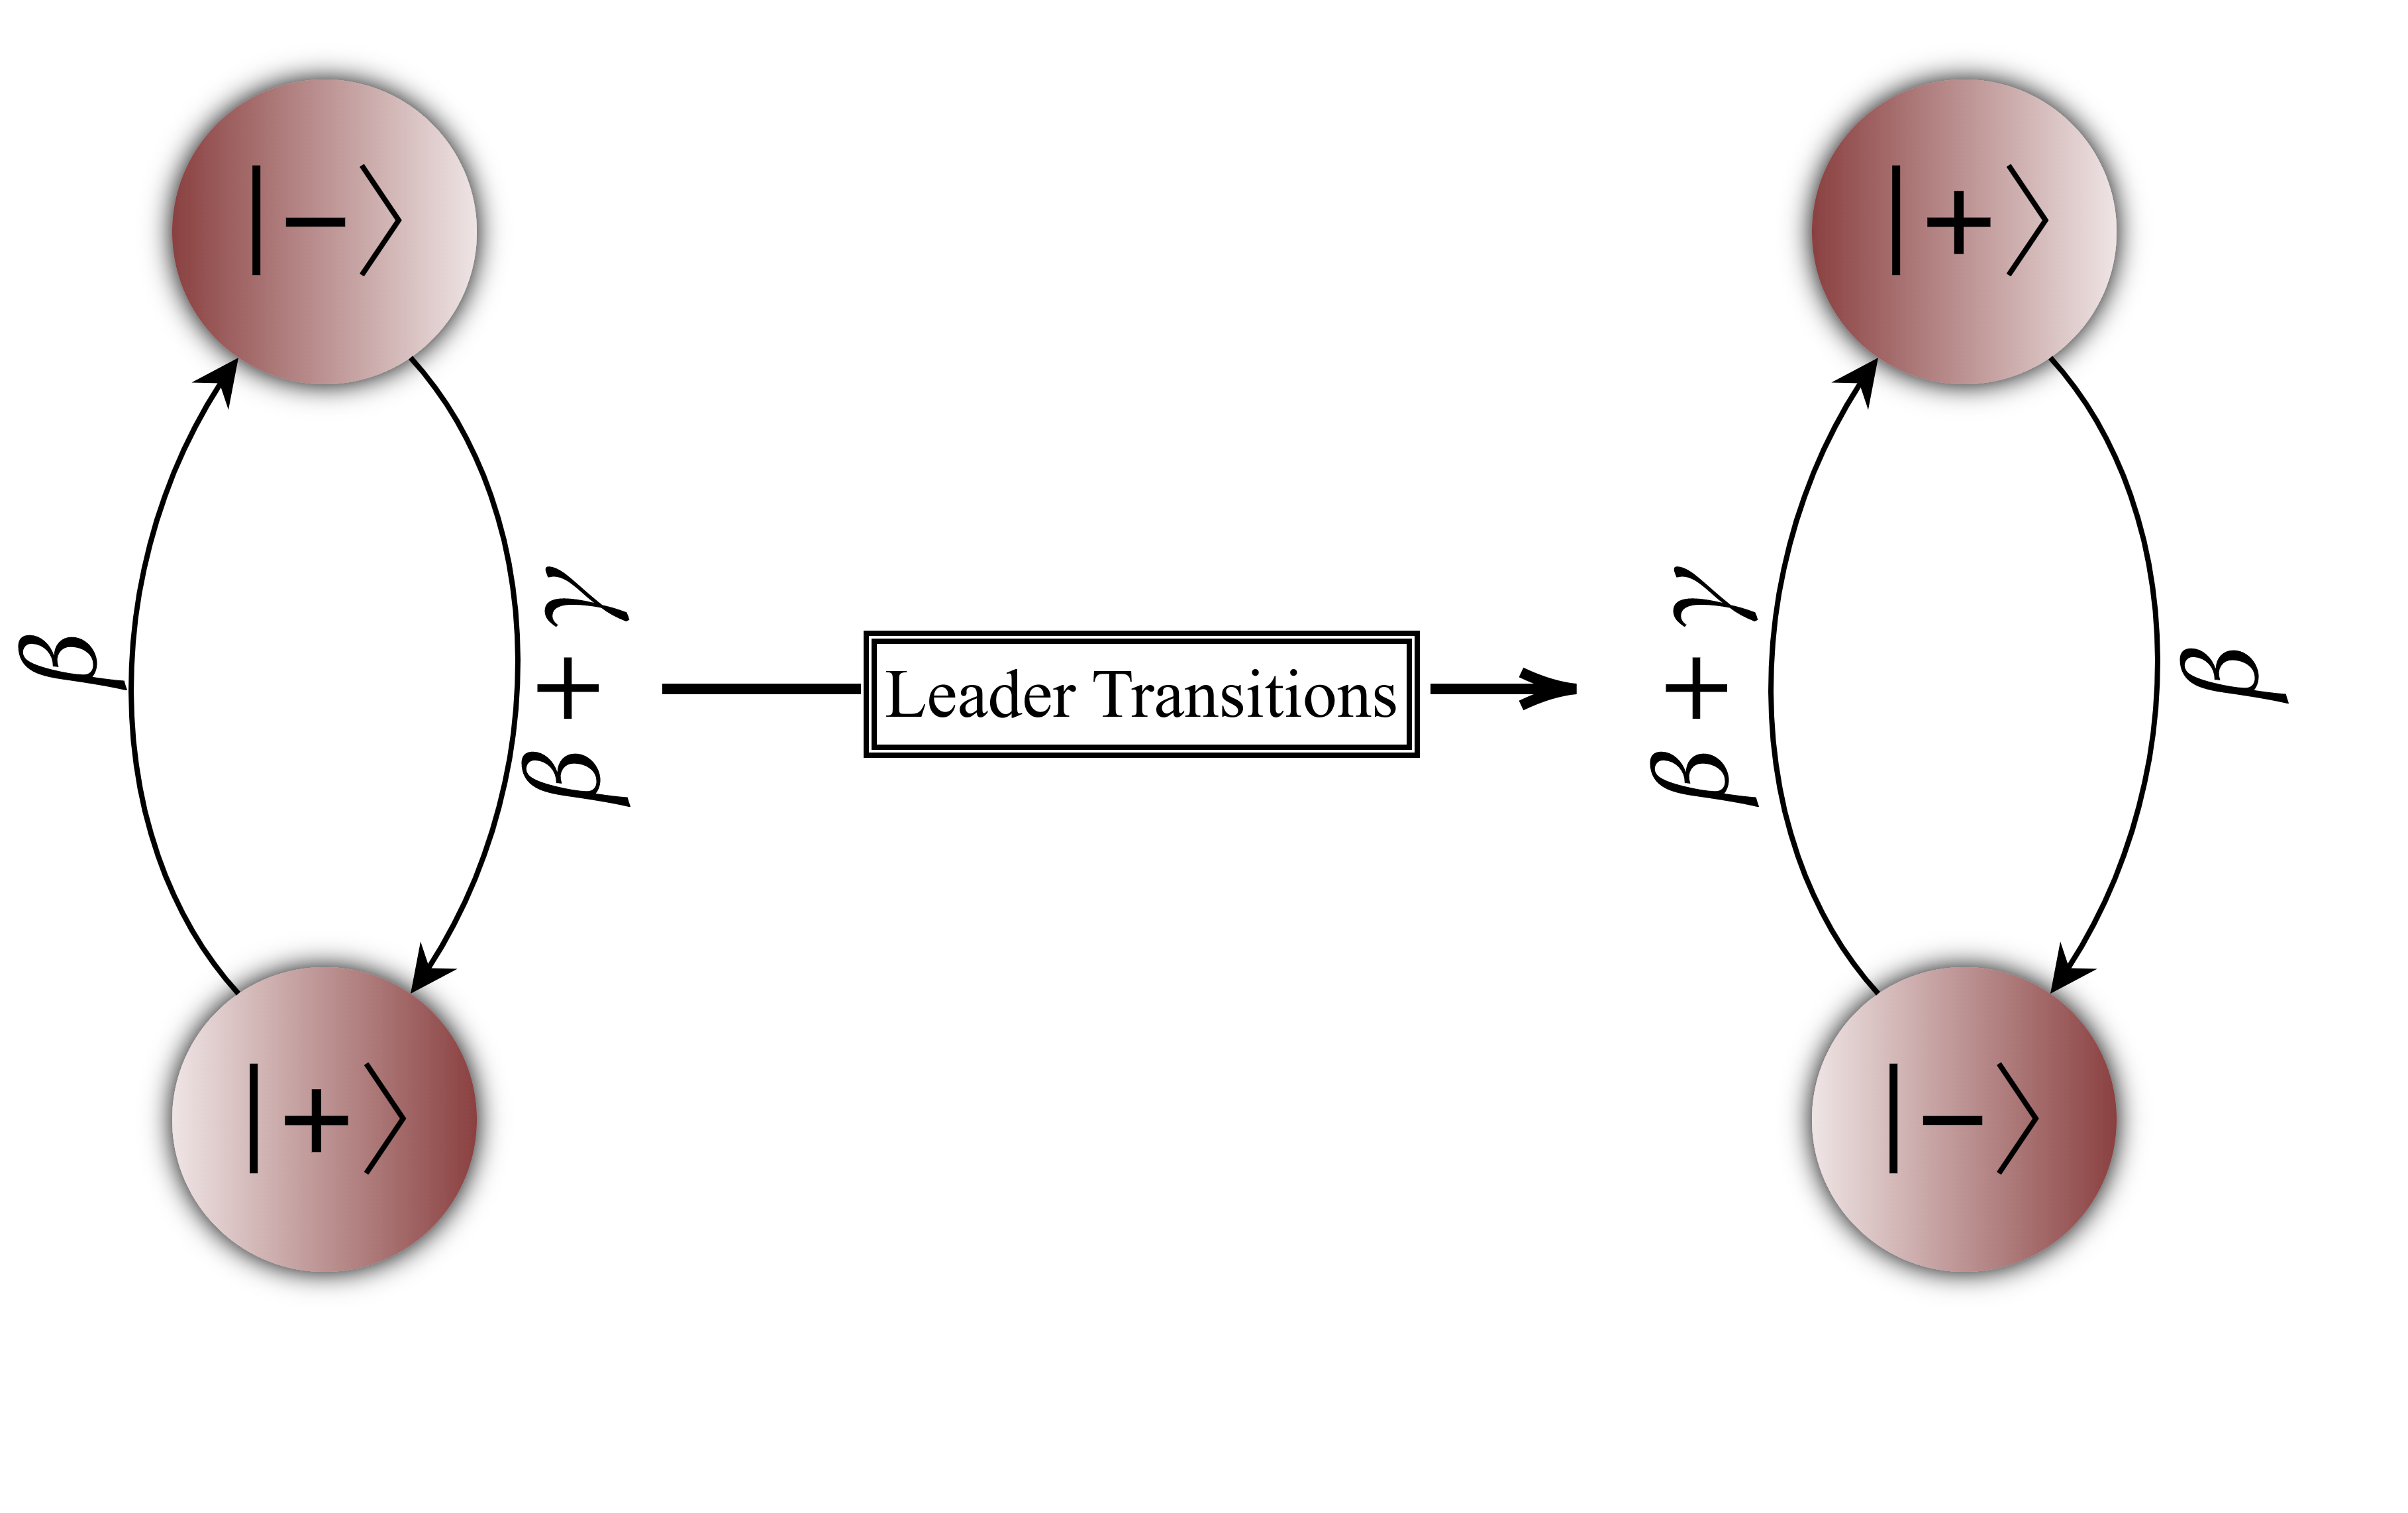
\includegraphics[width = 0.4\textwidth]{figures/follower_pov.png}
\caption{\footnotesize From the point of view of the follower particle, the states $\ket{1}$ and $\ket{2}$ are completely symmetric. The only asymmetry is brought about by the transitions of the leader which, in effect, switch the follower's preference for one state over the other. In this figure, the leader particle at first occupies the bottom state, meaning that the follower prefers it. Once the leader transition to the top state, the follower tends also to favour that state in its transitions. In this way, either of the state $\ket{1}$ or $\ket{2}$ can play the role of $\ket{+}$ as seen here.}
\label{follower-pov}
\end{wrapfigure}

With respect to the phase space, $W$ has the basis ordering $e_1 = \ket{11}$, $e_2 = \ket{21}$, $e_3 = \ket{12}$, and $e_4 = \ket{22}$, so that, for example, $W_{12}$ is the rate for the transition $\ket{21} \rightarrow \ket{11}$. As usual $\omega \in \Omega$ denotes a single path for the entire ensemble. We shall denote the leader's and follower's path by $\omega_A \in \Omega_A$ and $\omega_B \in \Omega_B$ respectively. Let $M = \mathds{1} + \tau W$ be the stochastic matrix of the discretised process. We intend to take the limit $\tau \rightarrow \rmd t$. Let us also write $M$ in block form 

\begin{align}
M = \begin{pmatrix} M_1 & M_2 \\ 
M_3 & M_4\end{pmatrix}.
\end{align}


The reason for this representation will become clear presently. We shall make the UL process non-Markov by hiding the leader's path from the observer, i.e. the observer shall only have access to $\omega_B$ and not to $\omega_A$. In this case, the observer cannot observe the states $\ket{11}$, $\ket{12}$, $\ket{21}$, and $\ket{22}$ individually. They may only observe convex combinations of the form $a\ket{11} + b\ket{21}$ and $a\ket{22} + b\ket{12}$. This coarse-grained system we will call the Unrequited Love (UL) process. When the observer measures $x_B = \ket{1}$ at time $t=0$, we deduce that the UL system is in the combination state $1/2 \ket{11} + 1/2 \ket{21}$. The normalisation factor is $1/2$ because the leader has no preference for either state. But note that this state can evolve non-trivially with time depending on the observed path $\omega_B$. The longer the follower is observed to stay in $\ket{1}$, the more likely it is that the underlying state of the granular UL system is $\ket{11}$, since, in a small time interval, the follower is less likely to transition away from $\ket{11}$ than from $\ket{21}$.\footnote{See the evolution equation for the states $\ket{w_1(t)}, \ket{w_3(t)}$ in Eqn. (\ref{w-evolutions})}

\begin{figure}
  \begin{subfigure}[b]{0.49\textwidth}
  \centering
  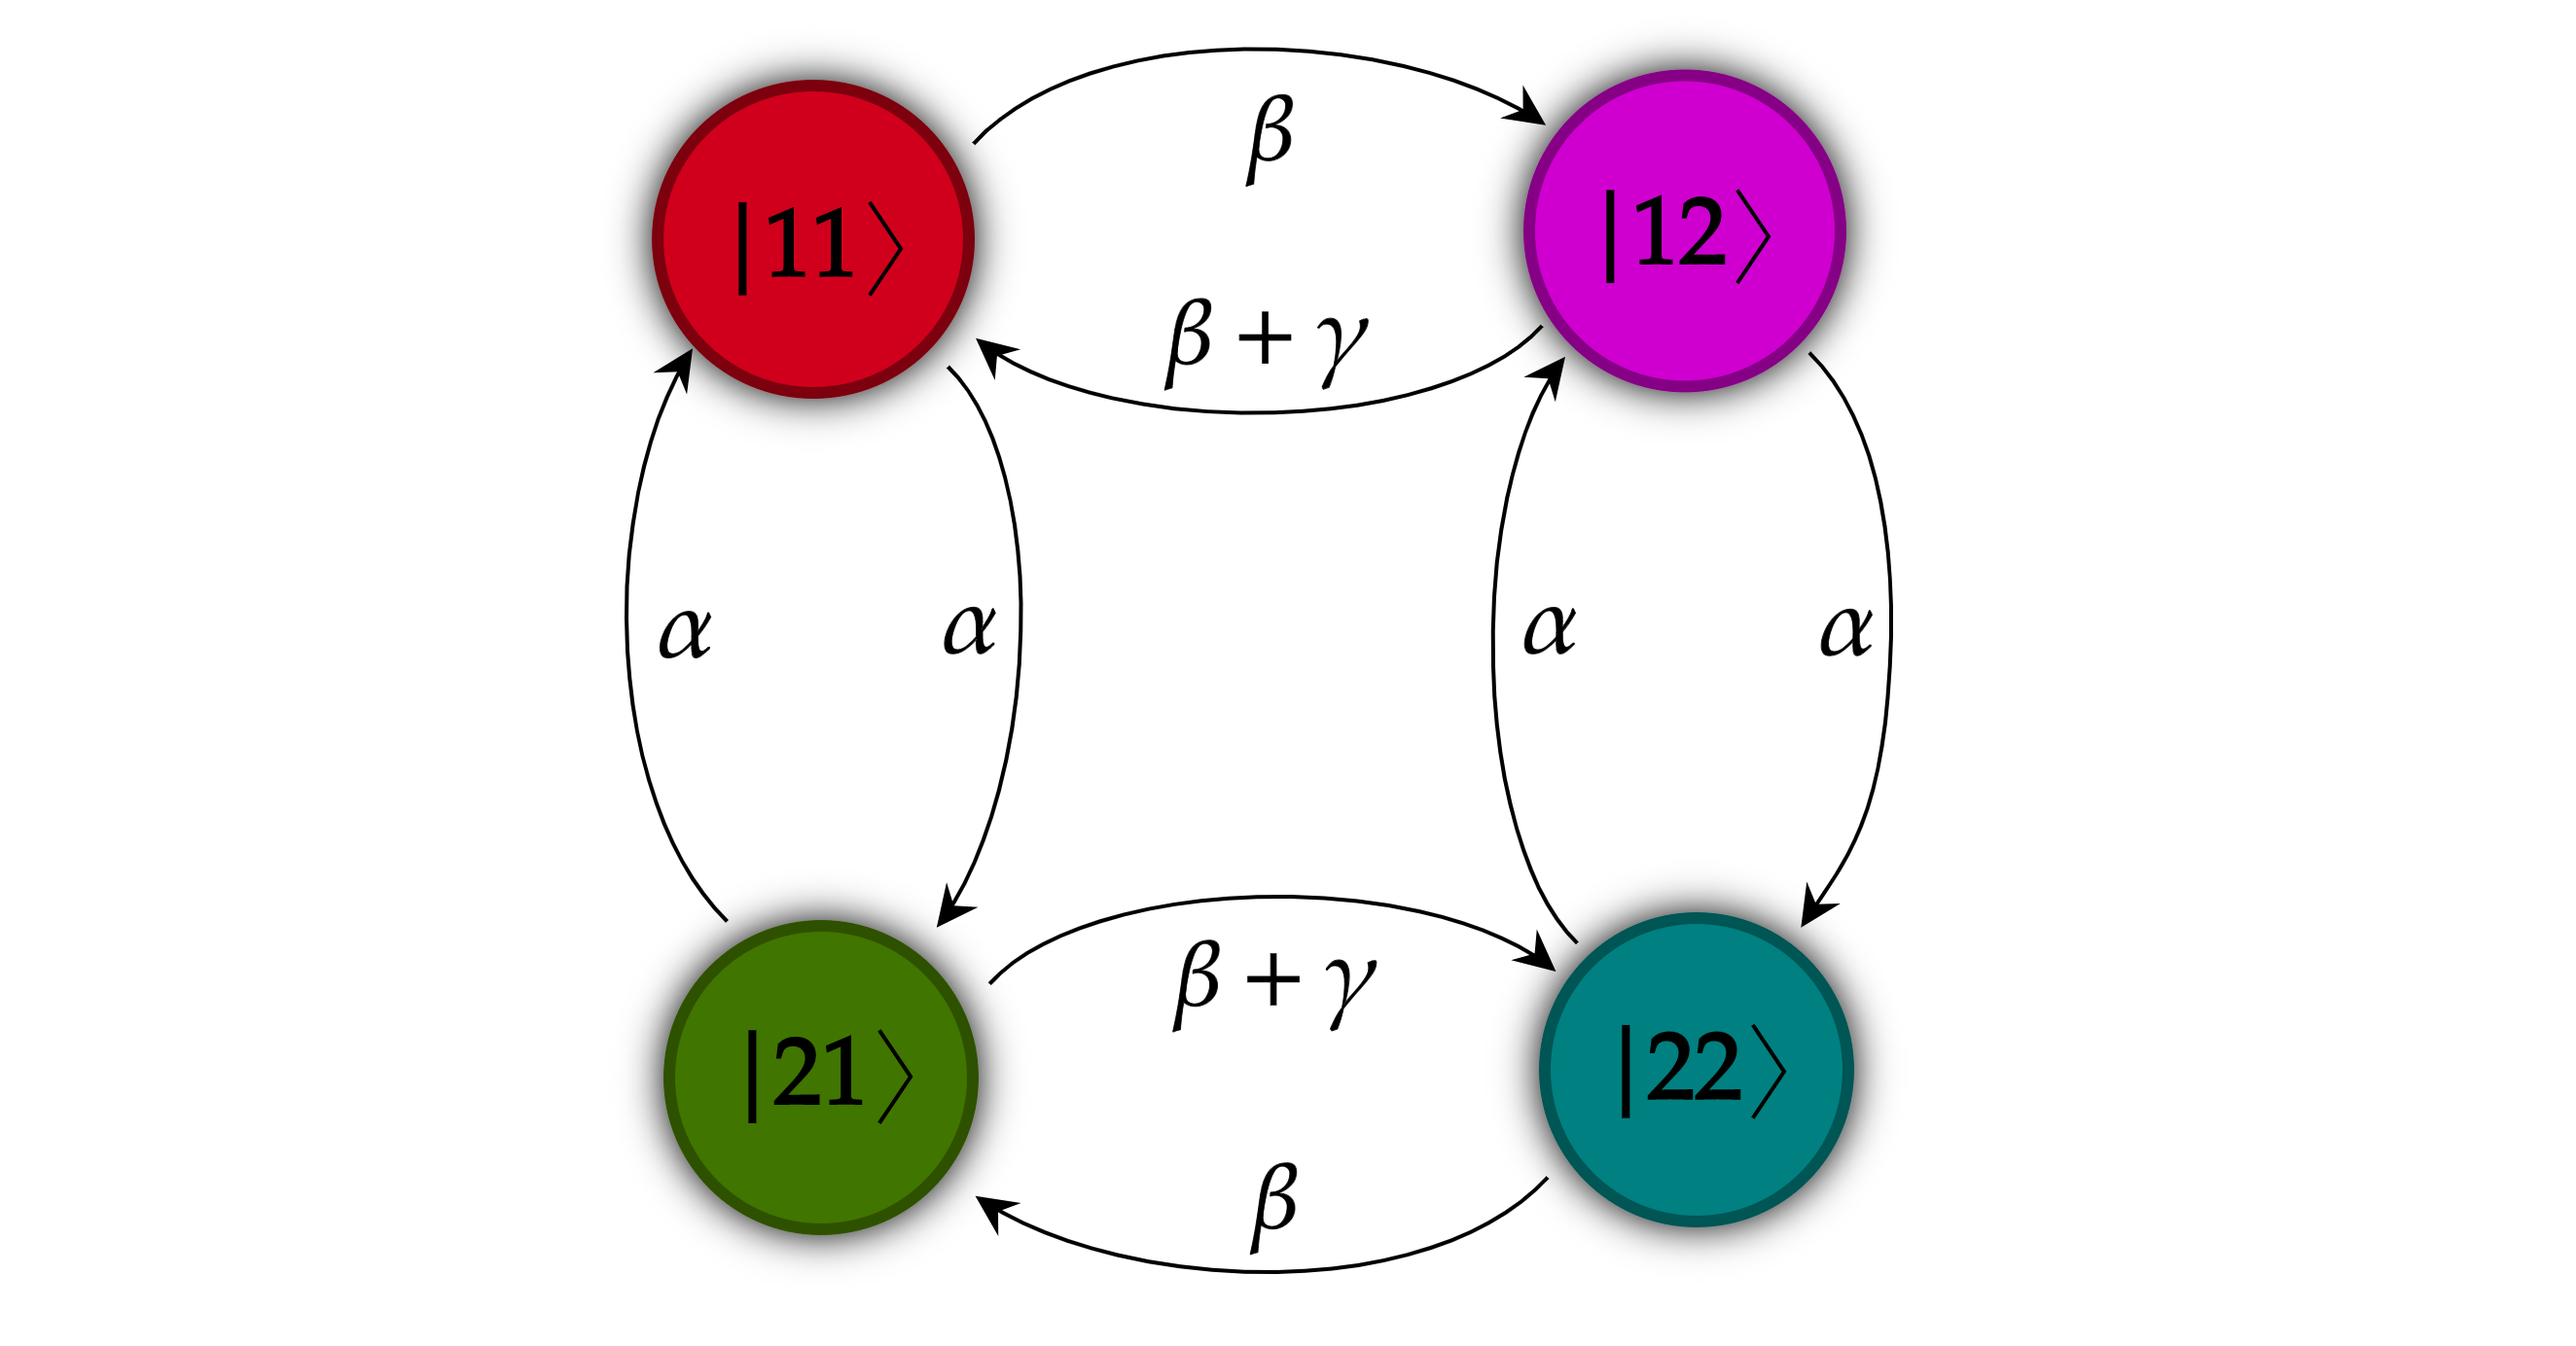
\includegraphics[width = \textwidth]{figures/UL_granular.png}
  \caption{Granular UL process}
  \label{granular_UL}
\end{subfigure}
\begin{subfigure}[b]{0.49\textwidth}
  \centering
  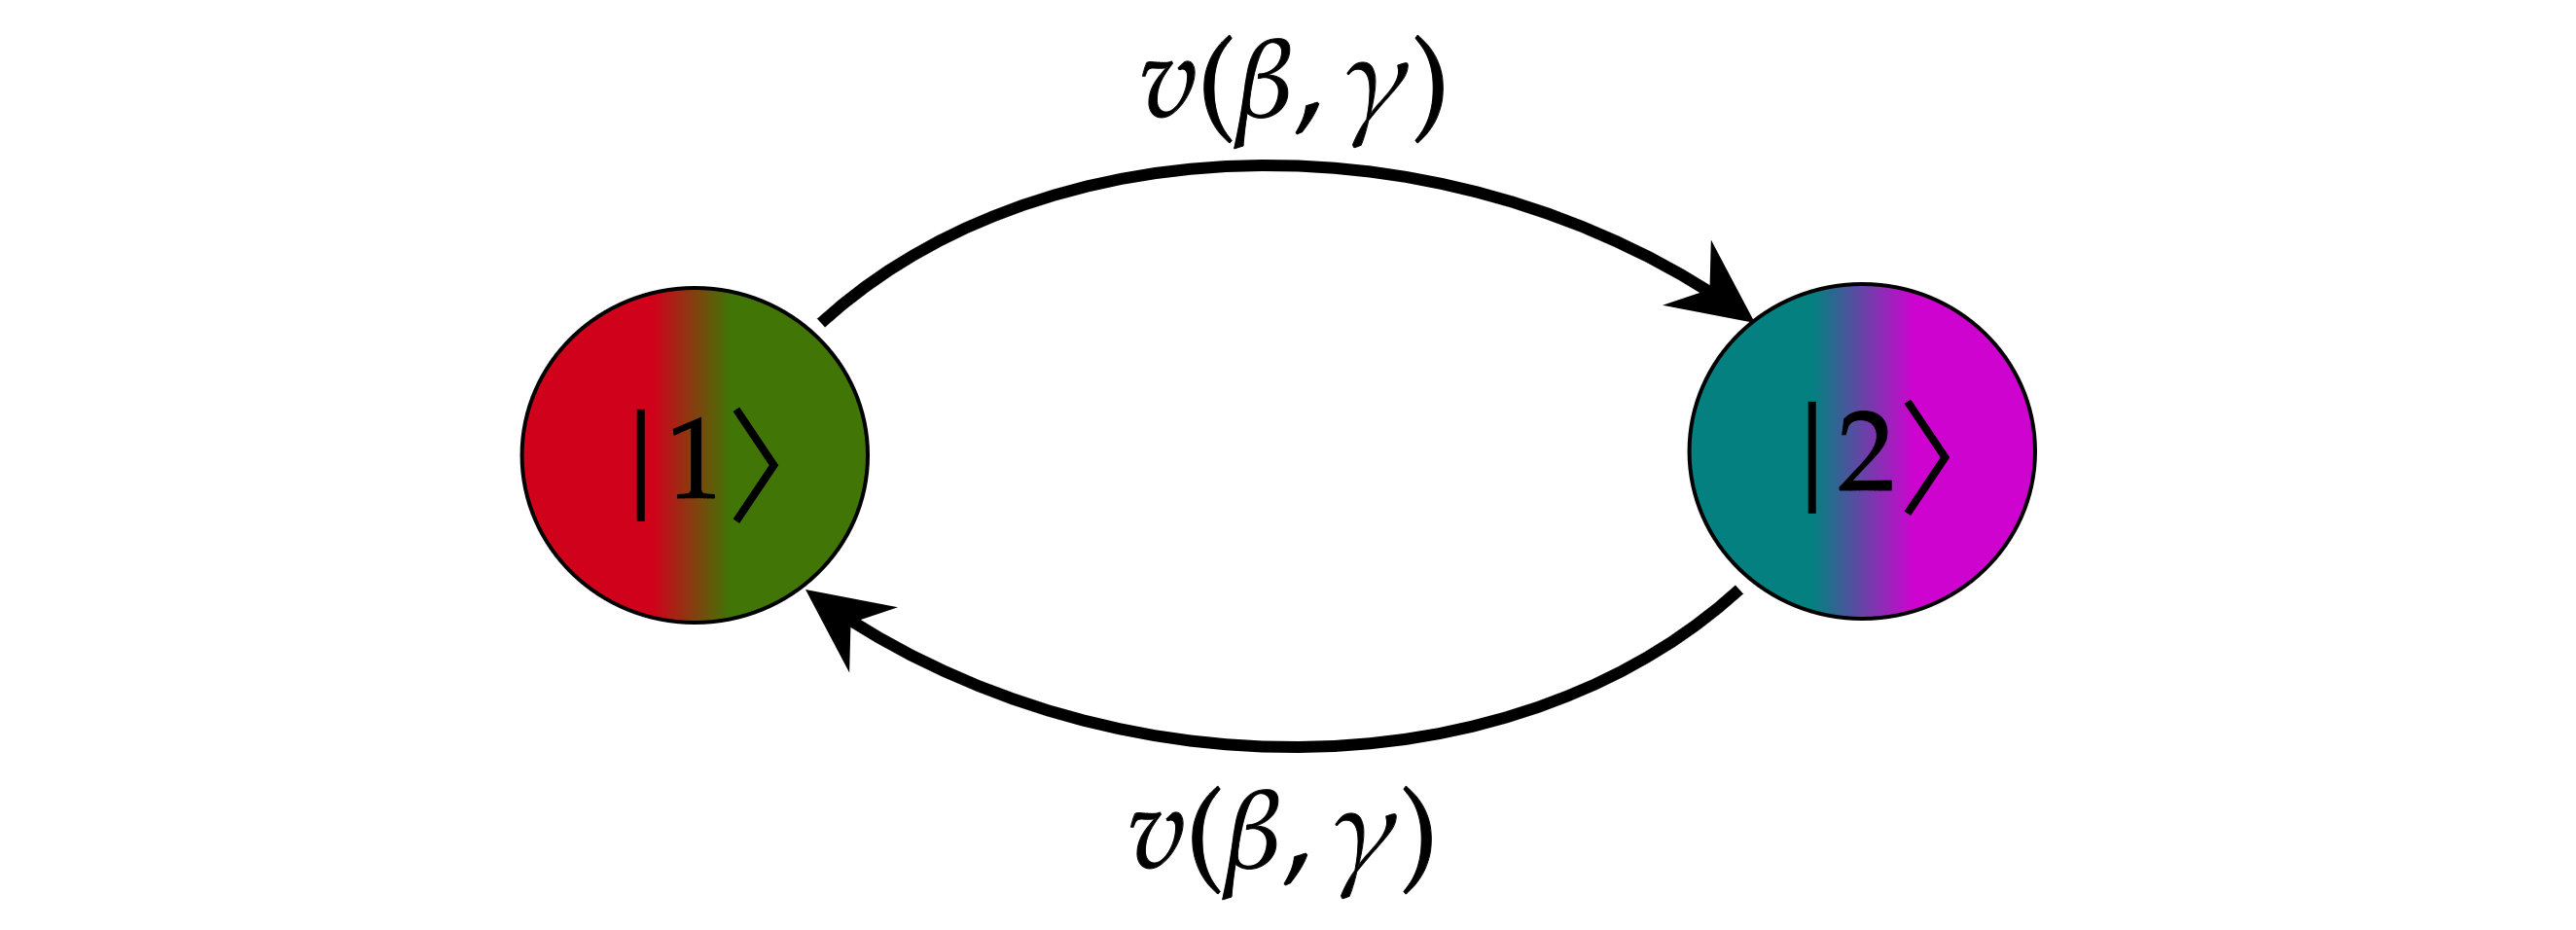
\includegraphics[width = \textwidth]{figures/UL.png}
  \caption{UL process}
  \label{coarse_grained_UL}
\end{subfigure}
\caption{\footnotesize Subfigure \ref{granular_UL} shows the layout of the granular UL system. The granular UL is a four-state continuous-time Markov chain. \ref{coarse_grained_UL} shows the states of the granular UL system collapsed together to give the UL process. In this picture, the follower hops between states $\ket{1}$ and $\ket{2}$ with some effective rate $v(\beta,\gamma)$. If one observes the UL system throughout the interval $[0,T]$, then the rate $v = v(t, \beta, \gamma)$ will be a process driven by the leader. See also Figure \ref{follower-pov}}
\label{system_desc_fig_UL}
\end{figure}


\subsection{Path Probability Derivation}

The probability of a path $(\omega_A, \omega_B)$ is 

\begin{align}
\bP(\omega_A, \omega_B) = \bra{x^1_Ax^1_B}M\ket{x^2_Ax^2_B}\ldots M\ket{x^N_Ax^N_B},
\end{align}

where $x^i_j$ is the state of particle $j$ at the $i$-th time step. Our aim is to derive the marginal probability of $\omega_B$ 

\begin{align}
\bP(\omega_B) = \sum_{\omega_A \in \Omega_A} \bP(\omega_A,\omega_B).
\end{align}

This will be  the probability accessible to the observer, since $\omega_A$ is hidden from them. We will perform this sum by summing over the possible trajectories of the leader at each step. For example, if $N=3$ and $\omega_B = \{\ket{1},\ket{1} , \ket{1}\} $, then

\begin{align}\label{path-prob-example}
\begin{split}
\bP(\omega_B) &= \frac{1}{2}\left (\bra{11} + \bra{21}) \right)M\left(\ket{11}\bra{11} + \ket{21}\bra{21}\right)M\left (\ket{11} + \ket{21} \right)\\
&= \frac{1}{2} \left (\bra{11} + \bra{21}\right) \begin{pmatrix}M_1 & 0 \\ 
M_3 & 0\end{pmatrix}M\left (\ket{11} + \bra{21} \right)\\ 
&= 1-2(\beta + \gamma/2)\tau + \mathcal{O}(\tau^2),
\end{split}
\end{align}

where we have used the fact that

\begin{align}
\ket{11}\bra{11} = \begin{pmatrix} 1 & & & \\ 
& 0 & & \\ 
& & 0 & \\ 
& & & 0\end{pmatrix}, \; \; \; \ket{21}\bra{21} = \begin{pmatrix} 0 & & & \\ 
& 1 & & \\ 
& & 0 & \\ 
& & & 0\end{pmatrix}.
\end{align}

The matrix blocks $M_1$ and $M_2$ contain all the information about transitions away from the states $\ket{11}$, $\ket{21}$, hence they appear when the CGUL system is in a combination of these states. Likewise, $M_2$ and $M_4$ will appear in the sum whenever the path indicates that the CGUL occupies $a\ket{22} + b\ket{12}$. Note also that the parameter $\alpha$ does not appear on the LHS of Eqn (\ref{path-prob-example}) since the nuisance paths of the leader have been summed over. 

Suppose now that the path $\omega_B$, composed of $t/\tau = N = \sum m_i$ total steps, is such that the follower spends $m_1$ steps in $\ket{1}$, $m_2$ steps in $\ket{2}$, then again  $m_3$ steps in $\ket{1}$ and so on until the path ends with the follower in $\ket{1}$ for $m_{L+1}$ steps (such that there are a total of $L$ transitions for the follower). Then we can write the path probability of $\omega_B$ as

\begin{align}
\bP(\omega_B) &= \frac{1}{2}\left(\bra{11} + \bra{21} \right)\begin{pmatrix} M_1 & 0 \\ M_3 & 0 \end{pmatrix}^{m_1-1}\begin{pmatrix} 0 & M_2 \\ 0 & M_4 \end{pmatrix}^{m_2}\ldots\begin{pmatrix} M_1 & 0 \\ M_3 & 0 \end{pmatrix}^{m_{L+1}-1}M\left (\ket{11} + \ket{21} \right) \\ 
\label{before-sum}
&= \frac{1}{2}\begin{pmatrix} 1 & 1 & 0 & 0\end{pmatrix}\begin{pmatrix} M_1 & 0 \\ M_3 & 0 \end{pmatrix}^{m_1-1}\begin{pmatrix} 0 & M_2 \\ 0 & M_4 \end{pmatrix}^{m_2}\ldots\begin{pmatrix} M_1 & 0 \\ M_3 & 0 \end{pmatrix}^{m_{L+1}-2}M \begin{pmatrix} 1 \\ 1 \\ 0 \\ 0 \end{pmatrix} \\ 
\label{after-sum}
&= \begin{pmatrix}1 & 1 \end{pmatrix} M_1^{m_1-1}M_2M_4^{m_2-1}M_3M_1^{m_3-1}\ldots M_3M_1^{m_{L+1}-1}\begin{pmatrix} 1 \\ 1\end{pmatrix} \\\label{path-density} &\eqqcolon \begin{pmatrix}1 & 1 \end{pmatrix}\phi\begin{pmatrix} 1 \\ 1\end{pmatrix}.
\end{align}

In Appendix \ref{appendix:recovering} we show how (\ref{after-sum}) follows from (\ref{before-sum}). If $t_i$ is the time of the $i$-th transition, we shall define $\tilde{t}_i = t_i - t_{i-1}$ such that $\sum_i \tilde{t}_i = t$. Here we use the convention $t_0 = 0$ and $t_{L+1} = t$. The $\tilde{t}_i$'s are the times spent in a state before transitioning. The limit $\tau \rightarrow \rmd t$ is equivalent to $N \rightarrow \infty$. Taking this limit while keeping the ratios $m_i/N$ fixed, for $j = 1,4$ we have 

\begin{align}
\lim_{N\rightarrow \infty} M_j^{m_i} =  \lim_{N\rightarrow \infty} ( 1+ \frac{t}{N}W_j)^{Nm_i/N} = e^{\tilde{t}_iW_j},
\end{align}

where $W_j$ is the $j$-th block of the matrix $W$ and $ \sum t_i = t$. On the other hand, for $j=2,3$, and in the limit of large $N$, we have $M_j \rightarrow W_j \rmd t $. For the rest of this section, we will abuse the notation to denote $\tilde{t}_i$ by $t_i$. So, in the large $N$ limit we have\footnote{See the derivation of the path probability in Section \ref{chapter:telegraph}}

\begin{align}
M_1^{m_i}M_2 \rightarrow \rmd t_i e^{t_iW_1}W_2, \; \; \; M_4^{m_i}M_3 \rightarrow \rmd t_i e^{t_iW_4}W_3.
\end{align}

Hence we have the limit 

\begin{align}\label{phi-limit}
\lim_{N\rightarrow \infty} \phi = \rmd t_1 \ldots \rmd t_L e^{t_1W_1}W_2e^{t_2W_4}W_3\ldots W_3e^{t_{L+1}W_1}.
\end{align}

In the sequel we will suppress the infinitesimals $\rmd t_1 \ldots \rmd t_L$ for brevity. Evaluating this product of matrices will give the density of paths that make $L$ transitions in time $t$. In general finding a closed form for (\ref{phi-limit}) is not trivial. We outline here our most promising approach. 

We will assume that $\gamma^2/\alpha^2, \gamma^2/\beta^2 \ll 1$ and we will ignore contribution of these orders. We first note the commutation relation

\begin{align}
\begin{split}
  e^{t_i W_4}W_3 &= W_3e^{t_i W_4} + \left[e^{t_i W_4}, W_3\right]  \\
  &=  W_3e^{t_i W_4} + (\alpha\gamma)\frac{2\sinh\left(\frac{t_i}{2}\sqrt{4\alpha^2+\gamma^2}\right)}{\sqrt{4\alpha^2+\gamma^2}} \begin{pmatrix} 0 && 1 \\ -1 && 0 \end{pmatrix}  \\
  &=  W_3e^{t_i W_4} + \gamma\sinh(\alpha t_i)  \begin{pmatrix} 0 && 1 \\ -1 && 0 \end{pmatrix} + \mathcal{O}(\gamma^2/\alpha^2).
 \end{split}
\end{align} 

Using this, and the fact that $W_2W_3 = \beta(\beta +\gamma)\mathds{1}$, we rewrite (\ref{phi-limit}) as 

\begin{align}\label{limit-phi-prod}
\begin{split}
\lim_{N\rightarrow \infty}\phi &= \left(\prod_{i=1}^{L/2}\left(e^{t_{2i-1} W_1} W_2 W_3
    e^{t_{2i} W_4} + \gamma\sinh(at_{2i}) e^{t_{2i-1} W_1} W_2\begin{pmatrix} 0 && 1 \\ -1 && 0 \end{pmatrix} \right)\right)e^{t_{L+1} W_1} \\
    &=  \left(\prod_{i=1}^{L/2}\left(\beta(\beta+\gamma)e^{t_{2i-1} W_1}e^{t_{2i} W_4} + \gamma(\beta+\gamma) \sinh(\alpha t_{2i})e^{t_{2i-1} W_1}\begin{pmatrix} 0 && 1 \\ -\beta/(\beta+\gamma) && 0 \end{pmatrix} \right)\right)e^{t_{L+1} W_1}.
\end{split}
\end{align}

By the binomial theorem, it follows that
\begin{align}
\lim_{N\rightarrow \infty}\phi = \left(\sum_{k=0}^{L/2} \beta^{L/2}(\beta +\gamma)^{L/2}\left(\frac{\gamma}{\beta}\right)^k\tilde{\phi}_k\right) e^{t_{L+1} W_1}
\end{align}

for appropriate matrices $\tilde{\phi}_k$. Each term in the above has a  coefficient proportional to $\gamma^k/\beta^k$ for some $k = 0, 1,\ldots L/2 $. Ignoring terms that have $k \geq 2$, we arrive at 

\begin{align} 
\lim_{N\rightarrow \infty}\phi = \phi_0 + \phi_1 + \mathcal{O}(\gamma^2/\beta^2),
\end{align}

where $\phi_0$ is the leading order term and $\phi_1$ is the sum of first order terms in $\gamma/\beta$. In Appendix \ref{appendix:recovering} we show that the contribution of $\phi_1$ to the path density (\ref{path-density}) is in fact $\mathcal{O}(\gamma^2/\beta^2, \gamma^2/\alpha\beta)$. It remains to evaluate

\begin{align}
\phi_0 = \rmd t_1 \ldots \rmd t_L \beta^{L/2}(\beta + \gamma)^{L/2}e^{t_1 W_1}e^{t_2 W_4}e^{t_3 W_1}\ldots e^{t_L W_4}e^{t_{L+1} W_1}.
\end{align}

Consider the basis of $\mathfrak{sl}(2)$ given by 

\begin{equation}
  H = \begin{pmatrix}1 && 0 \\ 0 && -1 \end{pmatrix}, \; \; X_+ = \begin{pmatrix}0 && 1 \\ 1 && 0 \end{pmatrix}, \;\; X_- = \begin{pmatrix}0 && -1 \\ 1 && 0 \end{pmatrix},
\end{equation}

and define the two families of indexed operators given by 

\begin{align}
  a_m = \left(\frac{m\gamma}{2\alpha}H + X_+ \right), \; \;
  b_m = \left(\mathds{1} + \frac{m\gamma}{2\alpha}X_-\right), \; \; m\in \bZ.
\end{align}

Notice that $a_m$ and $b_m$ are traceless for all $m$. Using this definition, we can write $W_1 = a_1 - (\alpha + \beta + \gamma/2) \mathds{1}$ and $W_4 = a_{-1} - (\alpha + \beta + \gamma/2)\mathds{1}$. Hence, by Proposition \ref{mat-exp-lemma}, `

\begin{align}\label{W1-exponential}
e^{t_iW_1} &= e^{-(\alpha +\beta+\gamma/2)t_i}\left(\cosh(\alpha t_i)\mathds{1} + \sinh(\alpha t_i) a_1 \right) + \mathcal{O}(\gamma^2/\alpha^2) \\
\label{W4-exponential}
e^{t_iW_4} &= e^{-(\alpha +\beta+\gamma/2)t_i}\left(\cosh(\alpha t_i)\mathds{1} + \sinh(\alpha t_i) a_{-1} \right) + \mathcal{O}(\gamma^2/\alpha^2).
\end{align}

Moreover, up to $\mathcal{O}(\gamma^2/\alpha^2)$, the following operator algebra holds\footnote{This means that, e.g., $a_ma_n = b_{n-m} + \mathcal{O}(\gamma^2/\alpha^2)$.}

\begin{align} 
a_ma_n &= b_{n-m} \\
  a_mb_n &= a_{m+n} \\
  b_na_m &= a_{m-n} \\
  b_nb_m &= b_{m+n}.
\end{align}

Using this algebra, any sequence of operators $a_{i_1}\ldots a_{i_N}$ where $i_n = 1, -1,$ is equal either to $b_m$ or $b_ma_1$ for some $m \in \bZ$. For example
\begin{align}
a_1a_{-1}a_{1} = (a_1a_{-1})a_{1} = b_{-2}a_{1}.
\end{align}

Note also that $a_ma_m = b_0 = \mathds{1}$, hence

\begin{align}
\begin{split}
b_ma_{\pm 1} &= b_ma_{\pm 1}a_{\mp 1}a_{\mp 1} \\
&= b_mb_{\mp 2} a_{\mp 1}\\
&= b_{m \mp 2}a_{\mp 1}.
\end{split}
\end{align}

Using (\ref{W1-exponential}) and (\ref{W4-exponential}) we can write for $\phi_0$

\begin{align}\label{phi0_factorised}
\begin{split}
\phi_0 &= \rmd t_1 \ldots \rmd t_L \beta^{L/2}(\beta + \gamma)^{L/2} e^{-(\alpha + \beta +\gamma/2)t}\bigg(\cosh(\alpha t_1)\mathds{1} + \sinh(\alpha t_1) a_1 \bigg)\bigg(\cosh(\alpha t_2)\mathds{1} + \sinh(\alpha t_2) a_{-1} \bigg)\\
&\quad \quad \ldots\bigg(\cosh(\alpha t_{L+1})\mathds{1} + \sinh(\alpha t_{L+1}) a_1 \bigg) \\ 
&= \rmd t_1 \ldots \rmd t_L \beta^{L/2}(\beta + \gamma)^{L/2}e^{-(\alpha + \beta +\gamma/2)t}\left (\prod_i \cosh(\alpha t_i) \right)\bigg( \mathds{1} + \tanh(\alpha t_1) a_1\bigg)\bigg( \mathds{1} + \tanh(\alpha t_2) a_{-1}\bigg)\\ &\quad \quad \quad \quad \ldots\bigg(\mathds{1} + \tanh(\alpha t_{L+1})a_1\bigg)  
\end{split}
\end{align}

If the leader has a very slow transition rate, then the distribution of time between two transitions of the follower approaches a double exponential distribution. When $\alpha$ is comparable to $\beta$, the underlying waiting-time distribution for the follower alternates depending on the state of the leader. The appearance of hyperbolic functions in $\alpha t_i$ indicates an averaging of these double exponential distributions. Indeed, when $\alpha \ll \beta$, we expect that $\alpha t_i \ll 1$ hence $\tanh (\alpha t_i) \approx 0$, and we are left with a double exponential distribution for each transition. It is doubtful, however, if considering the case $\alpha \ll \beta$ systematically will be of much physical relevance. Since we have already assumed $\gamma \ll \alpha, \beta$, imposing this new condition would constrain the analysis to those cases where $\gamma \ll \alpha \ll \beta$.

It is difficult to progress much further with the evaluation of $\phi_0$ into closed form. The chief difficulty is that, since the waiting times of the follower contain information about the position of the leader, the $t_i$ are not independent random variables. However, understanding products of the form $e^{t_1A}e^{t_2B}\ldots e^{t_LA}$ is of some mathematical interest (see for example \cite{friedland1994product, cohen1982eigenvalue}). So, in the interest of extending the analysis, we will recast Eqn. (\ref{phi0_factorised}) into a form which resembles a generating function, allowing combinatorial techniques to be used in future work. Define  $w_i = \tanh(\alpha t_i)$. Then From Eqn. (\ref{phi0_factorised}), we surmise that 

\begin{align}\label{phi0-prop-to}\small
\phi_0 &\propto e^{-(\alpha + \beta +\gamma/2)t}\left (\prod_i \cosh(\alpha t_i) \right)\bigg( \mathds{1} + \tanh(\alpha t_1) a_1\bigg)\bigg( \mathds{1} + \tanh(\alpha t_2) a_{-1}\bigg)\nonumber\\ &\quad \quad \quad \quad\ldots\bigg(\mathds{1} + \tanh(\alpha t_{L+1})a_1\bigg) \\ 
&= e^{-(\alpha + \beta +\gamma/2)t}\left(\prod_i \frac{1}{\sqrt{1-w_i^2}} \right)\left(\sum_{m = -L/2}^{L/2}c^0_m(w_i)b_m + \sum_{m = -L/2}^{L/2}c^1_m(w_i)b_ma_1\right)
\end{align}

where we have used the identity 

\begin{align}
\tanh^2 x + \sech^2 x = 1.
\end{align}

Recall that the RHS of (\ref{phi0-prop-to}) was obtained by expanding the product $e^{t_1 W_1}e^{t_2 W_4}e^{t_3 W_1}\ldots e^{t_L W_4}e^{t_{L+1} W_1}$. The equality 

\begin{align}\label{generating-function}
\bigg( \mathds{1} + w_1 a_1\bigg)\bigg( \mathds{1} + w_2 a_{-1}\bigg)\ldots\bigg(\mathds{1} + w_{L+1}a_1\bigg) =\left(\sum_{m = -L/2}^{L/2}c^0_m(w_i)b_m + \sum_{m = -L/2}^{L/2}c^1_m(w_i)b_ma_1\right)\label{generating-function}
\end{align}


resembles a generating function, with the chief difference that the $a_{\pm1}$'s do not commute. In every case, $c_m^k(w_i)$ is a polynomial in the $w_i$'s such that $w_j$ can only appear once in each term of the polynomial for fixed $j$. Further simplifications can be made if one assumes that the $t_i$ (and hence the $w_i$) are i.i.d. random variables. 

\subsection{Discussion}
The above analysis of the UL process demonstrates how a path-space approach to coarse-grained processes is in general highly non-trivial. This appears to be especially true of what we shall later venture to call `Lego brick processes' (See Section \ref{chapter:classification}).
Generating functions are an established method in combinatorics. They are usually used to count the subsets of a certain description from a set of given size. It is hoped that the method of generating functions can be extended to count permutations (rather than simply subset) of a given description. A method of counting the permutations of the operators $a_1$ and $a_{-1}$ in the expansion of the LHS of Eqn. (\ref{generating-function}) would provide a path forward for evaluating the coefficients $c^k_m(w_i)$ in closed form. 

An important limitation of the derivation above is that we have kept $L$ fix throughout. In particular, we have not considered the case of large $L$. At several stages in the derivation, we ignore terms of order $\mathcal{O}(\gamma^2/\beta^2)$ or above without considering how these terms scale with $L$. Consider, for example, the expression 

\begin{align}
\lim_{N\rightarrow \infty}\phi = \left(\sum_{k=0}^{L/2} \beta^{L/2}(\beta +\gamma)^{L/2}\left(\frac{\gamma}{\beta}\right)^k\tilde{\phi}_k\right) e^{t_{L+1} W_1}.
\end{align}

We go on to ignore terms in the above that are $\mathcal{O}(\gamma^2/\beta^2)$ or smaller. This means ignoring $\tilde{\phi}_{k}$ for $k \geq 2$. If $L$ is small, then this will not present any problems. However, taking note of Eqn. (\ref{phi-limit}), as $L$ grows large, $\tilde{\phi}_k$ grows as 

\begin{align}
\tilde{\phi}_k \sim \binom{L/2}{k} \sim (L/2)^k, \quad L \gg k.
\end{align}

This is because there are $\binom{L/2}{k}$ terms of order $\mathcal{O}(\gamma^k/\beta^k)$ in the expansion for $\phi$. So, in general, a perturbative approach to the path probabilities of the UL process will need to treat the limits of small $\gamma$ and large $L$ concurrently. If we confine ourselves to small observation time $t$, then the total probability of making $L \gg 1$ jumps is small, so the analysis presented heretofore holds. \newpage